% AI-assisted author-editing draft. Not a submitted or policy-certified paper.
% Official unmodified AAAI 2027 style is used provisionally; ICAPS-specific updates take precedence.
\documentclass[letterpaper]{article}
\usepackage[preprint]{aaai2027}
\usepackage[hyphens]{url}
\usepackage{graphicx}
\urlstyle{rm}
\def\UrlFont{\rm}
\usepackage{natbib}
\usepackage{caption}
\usepackage{amsmath}
\usepackage{algorithm}
\usepackage{algorithmic}
\usepackage{booktabs}
\usepackage{tikz}
\usetikzlibrary{positioning}
\frenchspacing
\pdfinfo{/TemplateVersion (2027.1)}
\setcounter{secnumdepth}{1}
\title{Progressive Topology Search with Substation Completion\\for Power Grid Control}
\author{Anonymous Working Draft}
\affiliations{}
\begin{document}
\maketitle

\begin{abstract}
Online power grid controllers use predictive simulation to compare topology interventions before execution. A global candidate order can interleave configurations of the same substation, so stopping after a favorable prefix or a reward plateau may leave a promising local decision unresolved; conversely, exhaustive evaluation spends computation on the entire eligible library. We propose a replaceable search layer that expands a ranked prefix using observed feedback and, after an extended-search stop, completes the unqueried configurations associated with the incumbent's substation. Under a common frequency order and hybrid controller, a four-date development study reduces candidate queries by 69.37\% and measured controller time by 13.11\% relative to exhaustive search, while completion reduces the worst complete-week cost increase from 4.81\% to 0.372\%. A separately frozen three-date study retains all failures and timing repeats, reduces queries by 83.54\% on the two dates with search and controller time by 6.09\% across all three dates, and satisfies the predeclared cost and survival screen; the first-safe reference is also competitive on these new dates, limiting claims of superiority.
\end{abstract}
\section{Introduction}

Power grid topology control changes the assignment of network elements to busbars to relieve congestion. An online controller must coordinate these discrete interventions with continuous redispatch, curtailment, storage, and restoration under changing load and generation. Predictive simulation makes this a deliberative control problem: before executing an action, the controller can inspect its forecast consequences, but each additional inspection incurs computation. Grid2Op provides a public environment for studying this repeated interaction \citep{grid2op}. For planning, the relevant issue is the allocation of computation to action evaluation inside an executing controller, rather than learning an action policy in isolation.


Existing hybrid agents combine continuous optimization with discrete candidate search, and learned rankers prioritize actions for simulation \citep{ljn2023agent,hassouna2025softgnn,dejong2025generalizablev1}. SoftGNN, for example, validates ranked candidates until it finds a forecast below a loading threshold \citep{hassouna2025softgnn}. These approaches already establish the usefulness of ranking and verification. Yet an action rank is not a certificate about the candidates that remain unevaluated. Topology actions form groups of alternative configurations at individual substations, and these alternatives need not be consecutive in a global order. A search can therefore locate a useful substation, observe a plateau in intervening candidates, and stop before inspecting another useful configuration at that substation.


This motivates a specific question: \textbf{can structural completion reduce the quality risk of early termination while retaining much of its computational saving?} Exhaustive search resolves every eligible alternative, but pays for the full pool. Returning the first verified action below a threshold is inexpensive when such an action appears early, but resolves only that threshold test. Progressive expansion provides an intermediate option; its stopping decision still leaves unqueried alternatives. We examine completion of the current incumbent's substation as a restricted additional search. We do not assume that substations are physically independent or that one-step reward predicts complete-episode cost.


Our method first simulates a ranked prefix, expands it in batches when the received feedback does not support stopping, and completes the incumbent's substation after a stop during extended search. The base controller, action order, admissibility checks, and shared compilation caches remain unchanged. The mechanism study demonstrates a case where 198 additional local evaluations recover the exhaustive reference's action after progressive search stops at 256 evaluations. Closed-loop evaluation then measures whether this repair is useful over a week, rather than treating a recovered action as sufficient evidence of long-term benefit.


The paper makes three contributions. First, it formulates and implements a search layer with explicit feedback permissions, stopping rules, and alias-aware structural completion. Second, it states the conditional incumbent-preservation property and exact additional-query cost of completion; these clarify the algorithm's scope without implying long-term safety. Third, it provides a common-order closed-loop comparison separating query reduction, measured controller time, episode survival, and benchmark operational cost. Four previously used dates support mechanism analysis; three separately frozen dates provide limited confirmation. The new-date results support savings relative to exhaustive search but do not establish consistent superiority over the first-safe reference. No new GNN or reinforcement learning training is required.


\section{Related Work}

\textbf{Hybrid and learned topology control.} The public LJN agent combines continuous control and topology intervention and supplies the base system and action library used here \citep{ljn2023agent}. SoftGNN learns preferences from multiple useful topology actions and validates candidates through simulation \citep{hassouna2025softgnn}. Its basic first-safe policy returns a do-nothing action if no candidate satisfies the threshold, while an extension uses restricted contingency-based search. Generalizable GNN topology control also studies verification and hybrid search variants \citep{dejong2025generalizablev1}. Thus neither ranking, simulation verification, disconnected-endpoint handling, nor hybrid continuous/discrete control is a novelty claim of this paper. We study an additional search policy inside that established interface. Our first-safe comparison adopts the published stopping principle but strengthens the exhausted fallback to the best admissible evaluated candidate; it is a controlled policy adaptation, not a complete reproduction of the published SoftGNN agent.


\textbf{Computation allocation in planning.} Deciding whether to perform another computation is a metareasoning problem. Bhatia et al. learn how to tune and terminate anytime planning \citep{bhatia2022metareasoning}, and bounded-optimal metareasoning explicitly considers the cost of deliberation \citep{milli2017metareasoning}. Our method is a fixed structural heuristic rather than a learned value-of-computation policy or a bounded-optimal controller. It allocates one-step simulator calls using the observed incumbent and a predefined configuration neighborhood. Its contribution must therefore be assessed as a concrete search specialization and its empirical behavior, not as the invention of adaptive stopping.


\textbf{Grouping and completion.} Searching alternatives associated with an incumbent is related in spirit to neighborhood exploration. Here the neighborhood is defined by original substation metadata and physical-action aliases after current-state canonicalization. Completion explores that neighborhood once, preserves the previous incumbent, and leaves alternatives at other substations potentially unresolved. This specification distinguishes the proposed policy from simply increasing a global prefix. Our experiments isolate completion from ranking and implementation reuse; they do not establish a general priority claim over all local-search or progressive-expansion methods.


\section{Problem and Search Interface}

At decision time t, the hybrid controller has public observation x and a base continuous action b. An original library I contains topology interventions, each with an identifier i and substation label s(i). Current legality and cooldown restrictions filter this library, and disconnected endpoints are handled by the shared preprocessing. Each remaining topology intervention is combined with b. Equal current physical action vectors are canonicalized; rep(i) maps an original identifier to its representative, and A denotes the ordered set of representatives. Original aliases and their substation labels are retained.


A dispatched query Q(x,b,a), for a in A, returns forecast reward r(a), maximum loading rho(a), and termination, legality, ambiguity, and exception flags. The policy can use the current public state, fixed metadata, and responses to queries it actually dispatches. It cannot inspect another policy's exhaustive results or an unqueried candidate's forecast. The experiment's exhaustive traces are available only to offline analysis.


The inherited admissibility rule is


\begin{equation}
0 < \rho(a) < \min\{\rho(x),\theta\},
\end{equation}

with no forecast termination, exception, illegal action, or ambiguous action. Here rho(x) is current maximum loading and theta is the threshold passed by the unchanged base controller. Admissible responses are compared lexicographically using


\begin{equation}
f(a)=\bigl(\operatorname{fp32}(r(a)),-i(a)\bigr),
\end{equation}

where i(a) is the canonical representative's retained library identifier. The float32 conversion and identifier tie break reproduce the base selection semantics. No admissible response yields no topology proposal; the unchanged base controller handles that outcome.


The episode-level objective is to reduce controller computation while retaining survival and acceptable operational cost relative to exhaustive candidate search. This operational cost follows the installed L2RPNSandBoxScore convention: a marginal generation-cost coefficient multiplies loss energy, absolute actual redispatch energy, \textbf{the change in curtailment energy}, and storage-throughput energy. It is a benchmark accounting quantity, not a production electricity bill or total curtailed energy. The query key f and complete-week cost are different quantities; improving f at one state need not improve the later trajectory.


\section{Progressive Search and Structural Completion}

\subsection{Overview}

FRAME combines three operations: establish an incumbent from a prefix, extend evaluation while feedback warrants further global search, and finish a restricted structural neighborhood before an extended-search return. The ranker supplies an order; it is not trained or changed by these operations. All principal experiments use the same author-frequency order, whose descending frequencies coincide with ascending frozen library identifiers.


\subsection{Progressive Evaluation}

The initial query set contains the first min(128,|A|) representatives. The best admissible response becomes the incumbent. If this prefix exhausts the pool, or if its incumbent has rho below the inherited safe threshold 0.9, the policy returns immediately. The threshold names a forecast criterion, not a safety certification.


Otherwise the policy extends the prefix in batches of at most 64. A batch that improves the incumbent's key resets a stale-batch counter; another batch increments it. Extended search stops when an incumbent is below 0.9, or after at least 256 queries and two consecutive batches without improvement. If no admissible incumbent exists, the policy continues to exhaustion. These constants were fixed in the development protocol and were not tuned on the separately frozen dates.


The plateau rule is a heuristic: recent non-improvement says nothing decisive about a later candidate. It buys computational savings by leaving part of the global order unresolved. Structural completion addresses a narrower risk within that unresolved part.


\subsection{Incumbent-Substation Completion}

Let C be the queried representatives when extended search ends, and let a\_C be its best admissible incumbent. If unqueried representatives remain, set s\_C=s(i(a\_C)). The completion set is


\begin{equation}
L=\{\operatorname{rep}(i)\in A\setminus C:s(i)=s_C\}.
\end{equation}

This definition includes a representative whenever any original alias belongs to the chosen substation. It does not discard an alias because its canonical representative has different metadata. FRAME queries every representative in L once and retains the best admissible key over C union L. The substation is fixed before completion begins: if a new incumbent is found, its substation is not recursively completed.


The initial safe-prefix return does \textbf{not} trigger completion. Therefore the method does not promise to resolve the returned action's neighborhood at every request. Completion is invoked only after extended search with an incumbent and remaining candidates. Figure 1 summarizes the distinction.


\begin{algorithm}[t]
\caption{Progressive Search with Substation Completion (FRAME)}
\label{alg:frame}
\begin{algorithmic}[1]
\REQUIRE Ordered representatives $A$, query interface $Q$, aliases and $s$
\STATE $C\gets Q(\text{first }\min(128,|A|)\text{ representatives})$
\STATE $a\gets$ best admissible response in $C$
\IF{$C$ exhausts $A$, or $a$ exists and $\rho(a)<0.9$}
  \RETURN $a$
\ENDIF
\STATE $stale\gets 0$
\WHILE{unqueried ordered candidates remain}
  \STATE Query next batch of at most 64; update $C$ and $a$
  \STATE Reset $stale$ if key improved; otherwise increment it
  \IF{$a$ exists and ($\rho(a)<0.9$ or ($|C|\geq256$ and $stale\geq2$))}
    \STATE Break
  \ENDIF
\ENDWHILE
\IF{$a$ exists and $C$ does not exhaust $A$}
  \STATE $s_C\gets s(i(a))$
  \STATE $L\gets\{\operatorname{rep}(i)\in A\setminus C:s(i)=s_C\}$
  \STATE Query $L$ once; update $a$ using the same key
\ENDIF
\RETURN $a$, or no topology proposal if none exists
\end{algorithmic}
\end{algorithm}

\subsection{Conditional Property and Query Cost}

\textbf{Proposition 1.} For a triggered completion with incumbent a\_C, assuming existing query responses are retained and only strict key improvements replace it, the selected action a\_after satisfies f(a\_after) $\geq$ f(a\_C). The additional query count equals |L|, and total queries are at most |A|.


\textbf{Proof.} The previous incumbent remains admissible in the saved response set. Selection over C union L therefore cannot yield a smaller lexicographic key than selection over C. By construction L contains only previously unqueried canonical representatives. A query registry prevents duplication, and no representative outside A is introduced. Hence completion adds |L| queries and the complete search purchases each member of A at most once.


The proposition is an implementation invariant, not an optimality theorem. A better action can remain outside C union L. Physical coupling between substations is retained by simulation, but is not solved by the neighborhood definition. FRAME may inspect the entire pool in the worst case, and it offers neither a sublinear worst-case bound nor a hard wall-clock deadline. Its single-state invariant does not imply non-degradation of full-week cost or survival.


\begin{figure}[t]
\centering
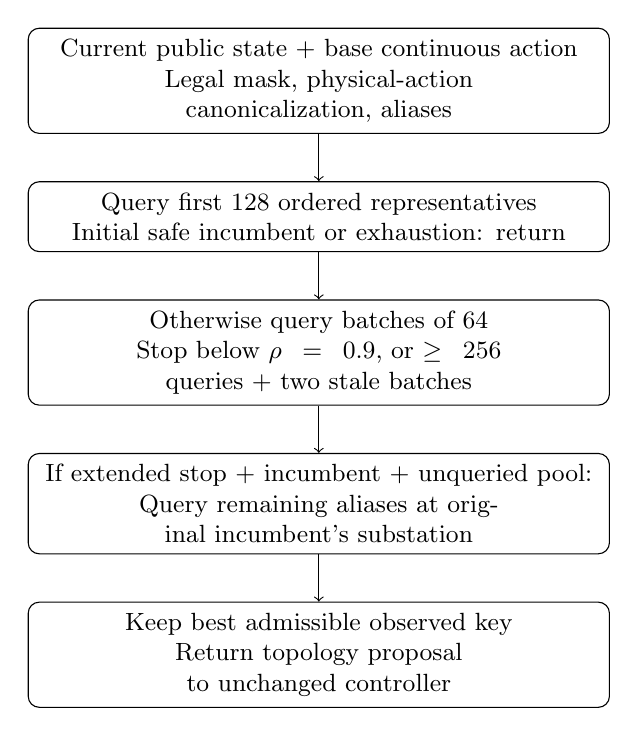
\begin{tikzpicture}[node distance=6mm, every node/.style={align=center,font=\small}, box/.style={draw,rounded corners,inner sep=4pt,text width=7.1cm}]
\node[box] (state) {Current public state + base continuous action\\Legal mask, physical-action canonicalization, aliases};
\node[box,below=of state] (prefix) {Query first 128 ordered representatives\\Initial safe incumbent or exhaustion: return};
\node[box,below=of prefix] (expand) {Otherwise query batches of 64\\Stop below $\rho=0.9$, or $\geq256$ queries + two stale batches};
\node[box,below=of expand] (complete) {If extended stop + incumbent + unqueried pool:\\Query remaining aliases at original incumbent's substation};
\node[box,below=of complete] (return) {Keep best admissible observed key\\Return topology proposal to unchanged controller};
\draw[->] (state)--(prefix);\draw[->] (prefix)--(expand);\draw[->] (expand)--(complete);\draw[->] (complete)--(return);
\end{tikzpicture}
\caption{Search interface and conditional completion. The initial safe-prefix return bypasses completion; a replacement action does not trigger recursive completion.}
\label{fig:framework}
\end{figure}
\section{Experimental Design}

\subsection{Controlled Policies and Environment}

We use the public l2rpn\_idf\_2023 environment, LightSim2Grid, and an LJN-derived hybrid controller \citep{grid2op,ljn2023agent}. The original library has 909 actions; masking and equivalence can reduce the current pool. The experiment compares four policies with a common frequency order, continuous controller, restoration cadence, admissibility rule, forecasts, and DC/safe-QP compilation caches:


\begin{table}[t]
\centering
\begin{tabular}{@{}p{.25\columnwidth}p{.69\columnwidth}@{}}
\toprule
Policy & Search behavior \\
\midrule
FULL & Evaluate all eligible canonical representatives; select the best admissible key. \\
FIRST\_SAFE\_BEST & Return the first admissible forecast below 0.9; on exhaustion retain the best admissible result. \\
NO\_LOCAL & FRAME's prefix, batches, and stopping, with structural completion disabled. \\
FRAME & Progressive evaluation followed by the conditional substation completion. \\
\bottomrule
\end{tabular}
\caption*{Shared-controller policy comparison. FIRST retains the best admissible response if its threshold is never met.}
\end{table}

FULL and FIRST\_SAFE\_BEST are the primary search references. NO\_LOCAL is a mechanism ablation. Shared caches are supplied to every applicable policy, so search savings are not obtained by withholding an optimization from FULL. Library order is a strong external frequency prior, not a random baseline. The author's original teacher-date exposure is unknown. No GNN inference or new training occurs in these two matrices.


The base implementation labels the hook N1; the counted queries are calls through that hook. This designation does not certify exhaustive N-1 security evaluation of every transmission line. Published PPO and SoftGNN adaptations from earlier experiments are supplementary system comparisons, not additional arms in the common-order policy matrix.


\subsection{Development and Frozen Confirmation}

The mechanism study uses four previously exposed date families: 2035-03-05\_0, 2035-06-25\_8, 2035-09-03\_4, and 2035-10-01\_5. Each policy has two serial timing repetitions, for 32 trajectories. These dates were used during development; they are not an independent generalization sample.


The final study uses all three date families still unaccessed in our local history: 2035-04-09, 2035-05-14, and 2035-11-19. All variants were excluded from local training and tuning. A fixed metadata-only hash rule selected primary variants 3, 14, and 0 before extraction of their episode payloads. The policies, order, thresholds, and balanced serial execution schedule were frozen before running the 24 trajectories. This is limited fresh-date confirmation on one grid, not a seasonally balanced sample or cross-grid validation. We do not merge its three families with development or historical model experiments as seven independent test families.


\subsection{Measurement and Implementation}

Let T\_m,d,j be measured controller wall time for method m, date d, and repeat j. It includes search preparation, ranking, simulation, and continuous-control work inside each controller decision. Initialization, physical environment steps, and artifact serialization are outside this interval. We average the two times within each date, then compute reductions relative to FULL and macro-average comparable dates:


\begin{equation}
\bar T_{m,d}=\tfrac12(T_{m,d,0}+T_{m,d,1}),
\end{equation}
\begin{equation}
S_T(m)=\tfrac1{|D_T|}\sum_{d\in D_T}\left(1-\frac{\bar T_{m,d}}{\bar T_{\mathrm{FULL},d}}\right).
\end{equation}

Here D\_T contains equal-horizon comparisons. Query reduction uses the same date-level approach but excludes zero FULL-query denominators. Complete-week cost change is (J\_m,d-J\_FULL,d)/J\_FULL,d and is reported only when both complete. Failures remain in survival and horizon reporting, rather than receiving credit for a shorter inexpensive episode.


A family passes the predeclared quality screen if it has no earlier failure and its comparable complete-week cost is at most 0.5\% above FULL. The final investment screen additionally requires at least two complete comparable dates, average controller-time reduction of at least 5\%, and a positive direction on at least two dates. These are finite experimental criteria, not tests of statistical equivalence or engineering safety. Timing repeats are not independent date families.


The host uses an AMD Ryzen 9 8940HX, Windows 11, Python 3.12.14, Grid2Op 1.12.5, LightSim2Grid 1.1.0, CVXPY 1.9.3, Clarabel 0.11.1, and OSQP 1.1.3. One serial CPU worker and single-thread numerical libraries are used. The per-episode engineering cap is 1,200 seconds, with a 60-second worker grace; batch caps are 6,000 seconds for development and 4,800 for confirmation. No cap-related truncation is counted as natural completion. Source, asset, configuration, and vector hashes are retained. Audits independently reconstruct saved feedback and public-state costs, but do not independently re-solve AC power flow.


\section{Results and Analysis}

\subsection{Quality and Computation}

Table 1 separates development from confirmation. Positive time and query percentages denote reductions relative to FULL; positive cost changes are worse. FRAME satisfies the quality screen on every evaluated date in both groups. Its query savings are much larger than controller-time savings because continuous control and other retained work remain in the decision loop.


\begin{table*}[t]
\centering
\begin{tabular}{@{}llrrrrr@{}}
\toprule
Set & Policy & Quality & Complete & Time & Queries & Cost \\
\midrule
Development & FULL & 4/4 & 3/4 & 0.00\% & 0.00\% & 0.000\% \\
Development & FIRST & 2/4 & 3/4 & 7.06\% & 51.45\% & +3.952\% \\
Development & NO\_LOCAL & 3/4 & 3/4 & 14.26\% & 71.84\% & +4.810\% \\
Development & FRAME & 4/4 & 3/4 & 13.11\% & 69.37\% & +0.372\% \\
Confirmation & FULL & 3/3 & 2/3 & 0.00\% & 0.00\% & 0.000\% \\
Confirmation & FIRST & 3/3 & 2/3 & -7.75\% & 89.24\% & -0.218\% \\
Confirmation & NO\_LOCAL & 3/3 & 2/3 & 9.38\% & 84.02\% & +0.014\% \\
Confirmation & FRAME & 3/3 & 2/3 & 6.09\% & 83.54\% & +0.014\% \\
\bottomrule
\end{tabular}
\caption{Date-level results. Positive time/query values are reductions; positive cost is worse. Confirmation query means use two nonzero-search dates.}
\end{table*}

FRAME retains most of NO\_LOCAL's development saving while reducing its worst complete-week cost increase from 4.810\% to 0.372\%. This supports completion as a useful repair in the development matrix. The uniform estimator in Section 5 yields 13.11\% controller reduction; the historical development report's 13.06\% averaged per-repeat ratios instead. The 0.0533 percentage-point difference is an aggregation change, not a new run or a changed quality verdict.


The frozen confirmation meets the declared investment screen, but its three dates are few and its timing dispersion is large. Table 2 exposes the individual FRAME results. The query reduction of 83.54\% is the average of the two nonzero-search dates; it is not an all-three-date query mean.


\begin{table}[t]
\centering
\begin{tabular}{@{}lrrrr@{}}
\toprule
Date & Steps & Cost & Time & Queries \\
\midrule
Apr. & 2017 & -1.328\% & 4.080\% & 5445 $\rightarrow$ 1012 \\
May & 747 & -- & 1.758\% & 0 $\rightarrow$ 0 \\
Nov. & 2017 & +0.014\% & 12.419\% & 2680 $\rightarrow$ 384 \\
\bottomrule
\end{tabular}
\caption{All frozen confirmation dates for FRAME; common failure and the zero-search date remain visible.}
\end{table}

The common June development failure occurs at step 1901; the common May confirmation failure occurs at step 747. FRAME introduces no earlier failure in these matrices, but passing a relative screen does not mean that it successfully controls every week.


\subsection{What Completion Repairs}

On the March development date, NO\_LOCAL's complete-week cost is 4.810\% above FULL, whereas FRAME's is 0.372\% above FULL. At the documented step 1733, NO\_LOCAL stops after 256 queries with action 26. Completing the incumbent's substation adds 198 queries and selects action 309, the same action chosen by FULL after 909 evaluations. Thus the structural neighborhood contains a consequential configuration that the global plateau stopping rule did not inspect. This is evidence of the skipped-local-configuration mechanism, rather than proof that all subsequent cost differences originate in this single step.


Saved-state qualification exactly reconstructs 90 prior FRAME calls; completion changes the selected action in 12. Those calls are mechanism checks, not 90 independent episodes. The development effect is concentrated in the March family. On the new April date, completion improves NO\_LOCAL's complete-week cost by only 0.00782\% of FULL; on November it does not trigger and FRAME and NO\_LOCAL have the same cost and physical path. The confirmation therefore does not reproduce a large local-completion quality event.


The ablation also reveals tradeoffs. Completion makes the macro controller reduction smaller than NO\_LOCAL's by 1.15 percentage points in development and 3.30 points in confirmation. It is additional work. Neither the invariant nor the experiment justifies describing the repair as cost-free.


\subsection{The First-Safe Reference and Timing Variation}

FIRST\_SAFE\_BEST fails the development quality screen on two of four dates, but passes on all three confirmation dates. On September development it has a lower cost than FRAME by 0.729\% of FULL. The October first-safe cost increase, 0.519\%, is close to the predeclared 0.5\% threshold and is reported without treating that small crossing as a large practical failure.


The confirmation's aggregate first-safe time is slower than FULL because its May repeats vary substantially, despite no topology search being called that week. It would be incorrect to attribute this difference to first-safe search. On the two dates with actual search, a post-run descriptive calculation gives controller reductions of 11.92\% for FIRST\_SAFE\_BEST and 8.25\% for FRAME. These subset calculations do not replace the frozen all-date primary estimator. They do show that the first-safe policy is a competitive alternative, and we do not claim that FRAME consistently outperforms it.


Repeated physical trajectories are identical within method and date, while measured time can differ. For April FRAME, the two controller times are 76.28 and 44.73 seconds; for May FIRST\_SAFE\_BEST they are 13.43 and 6.84 seconds. Process-CPU and continuous-optimization/compilation measurements also vary, while audited solver iteration totals agree. No power suspension event was observed, but instantaneous load and clock causes were not independently measured. We retain all repeats and report timing as observed point estimates. The current experiment does not establish a statistically reliable universal controller-speed improvement.


\subsection{Ranking and Implementation Attribution}

The common-order matrices establish that the reported framework behavior does not require a newly trained graph ranker. Historical GNN/PPO/SoftGNN adaptations remain available as supplementary system evidence, but use a different experimental role and are not pooled into this confirmation. Subsequent model revisions did not establish a stable incremental benefit over the strong author-frequency order. Ranking is consequently treated as a replaceable auxiliary component.


Compilation reuse has a separate engineering benefit and is supplied symmetrically to applicable arms. Percentages measured against an uncached controller are not added to the search reduction in Table 1. This distinction matters: an integrated controller can become faster for reasons unrelated to either graph representation or the proposed completion rule.


The development audit checks 63,616 saved physical rows and 70,358 matched query feedback items; confirmation checks 38,248 rows and 21,416 feedback items. All 16 development and 12 confirmation method-date pairs have identical repeated physical paths. These audits support accounting and implementation consistency; they neither enlarge the number of date families nor establish independent physical-solver validation.


\section{Discussion and Limitations}

The results support a restricted design lesson: when ranked actions interleave configurations of the same structural unit, a global stopping rule can leave a useful local decision unresolved. Completing that unit can recover a better observed action without returning to exhaustive global evaluation. In this application the unit is a substation, and the complete-week benefit is demonstrated most clearly on one development date. Applying this lesson elsewhere would require a justified neighborhood and closed-loop evaluation, rather than reusing the term completion as a generic guarantee.


The principal unresolved comparison is against inexpensive first-safe stopping. That policy is stronger on some dates and satisfies the new-date quality screen. Our study therefore supports a quality--computation tradeoff relative to exhaustive search and a specific repair mechanism, not a universal best controller. Parameter robustness has not been established, and the frozen constants are engineering choices rather than optimal schedules.


Only one grid and a small, locally selected date pool are evaluated. The held-out exclusion concerns our own training and tuning, not unknown exposure in the external action prior. Equal-horizon cost omits incomplete-week comparisons by design, and the common failures remain unresolved. The large timing variation limits the strength of time claims. The method has no global search-optimality, closed-loop safety, or hard real-time guarantee; its worst-case query count remains exhaustive.


\section{Conclusion}

We study progressive topology evaluation with incumbent-substation completion inside an established hybrid power grid controller. The policy uses only dispatched feedback, preserves its incumbent's observed key during completion, and explicitly accounts for the extra local queries. Controlled development results identify a skipped-local-configuration failure and show a useful quality--computation tradeoff; a small frozen confirmation retains query and measured-time savings relative to exhaustive search. Competitive first-safe results, shared failures, and timing variability delimit that conclusion. The contribution is a concrete search framework and its mechanism analysis, with learned ranking available as an auxiliary component.


\section{Broader Impact and Availability}

This is simulator-based decision-support research. Its forecast admissibility and relative-cost screen do not authorize deployment on an actual power grid or certify contingency security. Real deployment would require independent safety assessment, operating-rule verification, and operator supervision. The working evidence package contains source/configuration hashes, all per-run outcomes, candidate-query logs, and saved physical vectors. Preparing an anonymous, dependency-qualified release remains part of submission preparation; a source/table reproduction receipt is not a claim of independent full-simulator reproduction.


\begin{thebibliography}{6}
\bibitem[Bhatia et al.(2022)]{bhatia2022metareasoning}
Bhatia, A.; Svegliato, J.; Nashed, S. B.; and Zilberstein, S. 2022. Tuning the Hyperparameters of Anytime Planning: A Metareasoning Approach with Deep Reinforcement Learning. \emph{Proceedings of ICAPS}, 32:556--564. doi:10.1609/icaps.v32i1.19842.

\bibitem[de Jong, Viebahn, and Shapovalova(2025)]{dejong2025generalizablev1}
de Jong, M.; Viebahn, J.; and Shapovalova, Y. 2025. Generalizable Graph Neural Networks for Robust Power Grid Topology Control. arXiv:2501.07186v1.

\bibitem[Hassouna et al.(2025)]{hassouna2025softgnn}
Hassouna, M.; Holzh\"uter, C.; Lehna, M.; de Jong, M.; Viebahn, J.; Sick, B.; and Scholz, C. 2025. Learning Topology Actions for Power Grid Control: A Graph-Based Soft-Label Imitation Learning Approach. In \emph{Machine Learning and Knowledge Discovery in Databases. Applied Data Science Track and Demo Track}, 16022:129--146. doi:10.1007/978-3-032-06129-4\_8.

\bibitem[Lajavaness(2023)]{ljn2023agent}
Lajavaness. 2023. \emph{L2RPN 2023 LJN Agent}. Official source implementation. \url{https://github.com/lajavaness/l2rpn-2023-ljn-agent}.

\bibitem[Milli, Lieder, and Griffiths(2017)]{milli2017metareasoning}
Milli, S.; Lieder, F.; and Griffiths, T. 2017. When Does Bounded-Optimal Metareasoning Favor Few Cognitive Systems? \emph{Proceedings of AAAI}, 31. doi:10.1609/aaai.v31i1.11156.

\bibitem[RTE France(n.d.)]{grid2op}
RTE France. \emph{Grid2Op: A Testbed for Sequential Decision Making in Power Systems}. Official software, installed version 1.12.5; accessed October 13, 2026. \url{https://github.com/rte-france/Grid2Op}.
\end{thebibliography}

\end{document}
